\documentclass[UTF8, 11pt, oneside]{ctexart}

\usepackage{float}

\usepackage{geometry}
\geometry{a4paper,left=2cm,right=2cm,top=2cm,bottom=1cm}

\usepackage{graphicx}

\usepackage{hyperref}
\hypersetup{colorlinks=true, linkcolor=red}

\linespread{1.6}


\def\articletitle{人脑缓存太低,所以你家孩子绝不能死记硬背,因为肯定记不住}

\usepackage{fancyhdr}
\usepackage{ifthen}
\pagestyle{fancy}
\fancyhf{}
\setlength{\headheight}{14pt}
\fancyhead[R]{\ifthenelse{\value{page}>1}{\thepage}{}}
\fancyhead[C]{\ifthenelse{\value{page}>1}{\articletitle}{}}
\renewcommand\headrulewidth{0pt}

\usepackage{tcolorbox}
\tcbuselibrary{skins}


\newcommand{\zd}[1]{\textbf{\textcolor[RGB]{123,12,0}{#1}}} % 重点

\newcommand{\yh}[1]{% 引用
    \begin{tcolorbox}[enhanced,
        frame hidden, interior hidden,
        before skip = 5mm, left skip=10mm,
        borderline west={5pt}{0pt}{gray!50}]
        #1
    \end{tcolorbox}
}

\newcommand{\biaoti}[1]{% 标题
    \section*{#1}
}

\begin{document}

\begin{center}
    \LARGE{\articletitle\footnotemark}
\end{center}
\footnotetext{
    原文出自公众号“远方青木”的文章 《\href{https://mp.weixin.qq.com/s/H5zJJDr0nQIiwAYDYDxmkw}{\articletitle}》
}

\zd{今天就给大家闲聊点孩子教育方面的硬知识吧,希望能在教育孩子学习方面帮到大家。}

怎么样去学习才能记住大量知识,我有经验,也有办法。

但只是和你说这些办法是没用的,因为你无法理解这些办法为什么有效。

哪怕你信我,你孩子也不信我。

\zd{即便信,因为不知道原理,用起来效果也很差。}

\zd{所以我需要首先给你们讲解下人体大脑的构成。}

人类所有知识和智慧的硬件基础都是大脑,只有了解大脑运行的特点,你才有可能理解为什么有些办法可以让你轻易记住大量知识。

\zd{人类大脑的特点非常明显,用电脑专业名词类比的话,就是硬盘极大,缓存极小。}

大脑的神经元极多,理论上存储空间惊人,而实际上人类确实可以记住十几二十年来发生的很多很多事情。

这种存储能力是很多尖端电脑都达不到的,让很多科学家大为震惊,因此经常有什么人类还没有开发大脑潜力1\%的理论出现。

\zd{否则存储能力这么强大的你,为什么啥知识都记不住?}

但实际上人脑并不是只开发了1\%,而是开发了100\%。

\zd{之所以庞大的存储能力和你那可怜的知识储备不相匹配,是因为人脑的缓存低的惊人。}

什么叫缓存?

CPU可以瞬间读取的数据叫缓存,缓存里找不到数据就去内存找,还没有就去硬盘找,所以缓存极大的影响CPU的运算速度。

人类的缓存低到什么程度?

虽然你学会了算术,几千位的算术都不是难题,但人类的大脑却只能凭空计算二位数以内的乘除法。

除非掌握各种速算技巧,用投机取巧的办法得出计算结果,\zd{否则12乘以34等于几,这就是你可怜的大脑能算出的极限。}

你在大脑中模拟一张草稿纸,只能进行这个等级的运算。

\zd{至于三位数的乘法,比如说123乘以456等于几,你可怜的大脑就直接算卡壳了,算着后面的就忘记前面的,因为运算的数据量超过了你大脑的缓存极限。}

运算结果是56088,你的脑子算出来了吗?

\zd{别试了,小心直接把你可怜的大脑给算死机。}

但只要给你一张草稿纸和一支笔,让你在草稿纸上进行数学运算,成绩再差的学生都能轻易算出这个结果。

就算是1234乘以5678这种四位数乘法,乃至于更高等级的五位数乘法,凭借草稿纸你也可以轻易算出结果,而且毫无难度可言。

这种草稿纸就等于电脑的内存,极大的提升了你大脑的缓存上限,所以你才可以运算出三位数以上的乘法结果。

人脑是不是很奇妙?

\zd{你明明知道123乘以456怎么算,也可以凭借草稿纸轻易的算出结果,但不给你草稿纸,你就是算不出来。}

\zd{你的大脑就这么点硬件条件,而且各学科的顶级专家也不会比你强哪去。}

数学如此,语文也是如此。

《滕王阁序》是中国语文的必背课文,无数中国孩子考试时的梦魇。

此文极长且需要全篇背诵,还是晦涩的文言文,很多孩子们做梦时都在背这篇课文,结果考试的时候还是记不住。

\zd{想全篇背诵《滕王阁序》,不掌握技巧是绝对不可能的事情,因为《滕王阁序》全篇的信息容量,已经超过了人脑缓存极限。}

没有任何人类可以强行背诵《滕王阁序》全篇,我说的是任何人类,因为你大脑的硬件条件不允许你这么做。

\zd{所有能背诵《滕王阁序》全篇的人都掌握了记忆技巧,只不过有些是主动领悟的,有些是在漫长而痛苦的背诵中被动领悟的。}

还有一些人至死都无法领悟,那考试的时候碰到《滕王阁序》就要丢分。

丢分就丢分了,不会就是不会,没办法。

觉得自己记忆好的人,我考一下你们。

《滕王阁序》里最出名的一句话,是“落霞与孤鹜齐飞,秋水共长天一色。”。

这句话的后面一句是什么?

绝大多数人都记不住了,有些人甚至考试结束后几天就记不住了。

但我只要和你说“落霞与孤鹜齐飞”,你基本上都能回忆起“秋水共长天一色”。

甚至只要说一个落霞,你马上就能接出整句话。

\zd{因为人脑的缓存极限,其实就只有一句话多一点,最多不超过2句话。}

\zd{所以你记忆这么一句话是可以的,记两句话就够呛。}

\zd{整篇滕王阁序在你的大脑中,实际上是被割裂为几十句话后零散的记住。}

所以你记住全篇的每一句话都很简单,哪怕忘了,点个开头就能立刻想起全句,但背诵全篇就超级困难,困难的无以复加。

\zd{把被割裂为几十处的零散知识点串起来,你就能背诵滕王阁序全篇。}

\zd{如果串不起来,你就绝对无法背诵全篇。}

\zd{死记硬背能记住滕王阁序全篇是绝对不可能的,没有任何人类能做到。}

\zd{不是说你不行,而是说所有人类都不行。}

“落霞与孤鹜齐飞,秋水共长天一色”的下一句是“渔舟唱晚,响穷彭蠡之滨”。

点你“渔舟”两个字,你就可以立刻背出下一句。

因此想同时背出这两句话,你就需要在第一句的后面自己加一根锁链,把长天一色和渔舟进行捆绑记忆。

背到长天一色,直接想起渔舟,然后前面的东西直接遗忘,移出大脑缓存,开始回忆渔舟后面的东西。

同理在你背到“彭蠡之滨”的时候,立刻联想到大雁,然后就可以背出下一句“雁阵惊寒,声断衡阳之浦”。

\zd{几十个这样的小锁链组合在一起,配合你记住的几十个零散语句,就可以支撑你背诵滕王阁序全篇。}

\zd{这个锁链阵没有学术名称,是我个人定义的,我将其称之为文章脉络。}

\zd{不背下脉络,单纯去硬背,能背下滕王阁序纯属做梦。}

而脉络也需要背诵,如果比较长,那就需要一个更小的锁链去记住这个大锁链,因此背下文章脉络也需要脉络。

如此反复,直到最小的脉络大概只需要花费你3~5秒不到的时间记忆为止。

所以人类可背诵的文章长度,是有极限的。

\zd{当最小的脉络等于你大脑天生的缓存极限时,就达到了你可背诵的理论极限文章长度,再多你肯定记不住。}

你天生缓存越大,极限记忆长度就越强,但不同人类之间的缓存差距再大也没多少。

当然如果你不懂的记忆办法,只知道死记硬背,那你缓存哪怕达到了人类的最大值也不如普通人类的记忆能力强。

\zd{至今没有任何人类大脑的数学运算缓存能力能超过一张草稿纸,你天赋再强也就这个极限。}

\zd{只能说在同样掌握草稿纸的前提下,缓存能力越强的人,运算速度越快,运算极限越高。}

在文学领域,关于文章脉络的记忆,也有\zd{低级、中级和高级之分。}

作为学生,你只需要低级的文章脉络就足够了,因为只需要背诵,不需要其他。

\zd{在学生阶段,低级脉络反而是最有用的,能最快速度提升成绩,其他等级的脉络没有用,学生也不需要好高骛远去想这些。}

\zd{但当你步入社会之后,低级的脉络记忆是没有用的,没有任何人会对你是否能背诵滕王阁序感兴趣,能背这个也不会让你的月薪增加一毛钱。}

\zd{这个时候,你就需要中级的脉络记忆,以及高级的脉络记忆。}

这东西没有任何人去教,只能靠你自己去领悟,对学生没用,但对成年人有用。

\zd{我领悟的是我自己的东西,你能不能直接用我不知道,因为每个人的大脑都是独一无二的,有相通性但肯定不完全一样,越高级的大脑运转办法越讲究自己领悟。}

\zd{今天我讲给你听,你能借鉴多少算多少。}

以《滕王阁序》为例,所谓中级脉络记忆,就不是简单的记住长天一色后面有个渔舟,彭蠡之滨后面有个大雁了,\zd{而是你要记住王勃当年写《滕王阁序》时的感情,行文理由,文章逻辑推进过程。}

王勃为什么要这么写?写“邺水朱华,光照临川之笔”时后面为什么非要写“四美具,二难并”?

理解这些,记住这些,你对《滕王阁序》的理解和记忆就达到了第二档次,也就是中级脉络记忆。

这么记有什么好处?

好处那可就太多了。

首先在低级脉络的记忆办法里,你除了记住脉络之外,还必须要记住几十处零散句子,没有那几十处零散句子的背诵,你光有低级脉络是没用的。

但是在中级脉络里,零散句子是记忆量是可以大幅压缩的,只记住一点点句子就可以了。

\zd{中级脉络领悟到极限,《滕王阁序》你甚至可以一句话都不背。}

\zd{因为低级脉络讲究的是记忆《滕王阁序》的形。}

\zd{而中级脉络讲究的是记忆《滕王阁序》的魂。}

掌握中级脉络后,你是可以复刻《滕王阁序》的。

虽然我背不下来《滕王阁序》全篇,但我可以自己写一个差不多的。

能背下的零散句子就填充进去,背不下来的就自己脑补一句放进去。

\zd{你对《滕王阁序》的理解越深,脑补出来的假句子读起来就越像真的。}

这么做在学校考试阶段是肯定要扣分的,因为老师要求一字不差,但踏入社会后是大大加分的。

\zd{中级脉络发展到最后,你的脑补能力会提升到极致,然后你就可以从头到尾脑补出一个和《滕王阁序》极其类似,但并不完全相同的文章。}

\zd{此时你就从一个学生,步入了文学创作的最低级门槛。}

著名的《沁园春·雪》,以及所有的沁园春开头的诗词,都是以唐朝的沁园春词牌为基础进行创作的。

\zd{韵律一样,脉络一致,你脑补出不同的填词,就是不同的沁园春。}

\zd{脑补出再烂的填词,你也算一个诗人,不算那种只会背诵的学生了。}

填词越优秀,写出的沁园春越伟大。

\zd{所有文学家,都是从分析、提取、学习、吸收中级脉络开始锻炼的。}

\zd{无一例外。}

最多就是大家对各自领悟办法的命名不一样而已。

至于文学的高级脉络,这个听起来好像就更虚了。

\zd{简单的说,这时候你可以抛弃所有基础知识点的背诵,专门记忆行文套路、世界运转规律、各领域疑难问题的推理和分析过程,并不断打磨、优化和记忆那玄之又玄的所谓“写作感觉”。}

\zd{这些东西全部提取自中级脉络,每一个中级脉络里面都蕴含高级脉络的所有零件。}

\zd{拥有大量文章、文体的中级脉络后,打碎它们,提取零件,并重新凝聚成一个新的整体,你就形成了自己高级脉络的雏形。}

此时你就是一个真正的作者,段位高那种只会背诵的学生不知道多少级。

高级脉络一旦形成,只需要记住这个脉络,你就可以源源不断的写文章,感觉文学相当简单,而且文章信手拈来,文体也绝不局限于沁园春词牌或者某个爆款刷屏文的固定格式。

\zd{形成自己高级脉络的人,没有固定格式,更绝不会拘泥于中级脉络,想怎么写就怎么写,写啥东西都是文章。}

\zd{你的高级脉络形成时是什么样子,你的文风就是什么样子。}

平时随便找素材,找到什么素材往你脉络里一填,那就是一篇文章,堪称流水化批量生产,根本不用苦思冥想拼命拽头发。

在这类作者眼里,一篇文章除非有独特的观点或者新奇的视角,否则都不算得意文章。

在高级脉络里单纯填素材的文章,普通人已经觉得很优秀了,普通作者更是觉得全文流畅不已,相当精彩。

但在这种等级作者眼里,这叫水文,一般拿来凑数用,毕竟独特观点不太可能天天悟出来,但很多时候需要天天更新。

我也经常水文,所以对这个很清楚。

也因此顶级作者的文章是无法伪造的,基本上一眼就能看出是不是他写的。

因为没有他脉络的人,永远写不出他的文风,强行按中级脉络去拆解模仿,仿出来的文章质量极低,差别极大,简直就是天地之差那种。

就算是顶级作者的水文,其精彩程度都不是中段位作者能模仿出来的。

\zd{这就是所谓的学我者生,似我者死。}

别说别人揣摩中级脉络后模仿文风,就算这个顶级作者切换一个领域去写文章,如果他本人没有形成这个领域的高级脉络的话,那文章质量也会刷刷地掉。

当然有些作者实力极强,形成了多个领域的高级脉络,所以可以跨领域写作,但不同领域的高级脉络领悟程度肯定有所差别,所以在不同领域发挥的实力也不尽相同。

比如说我自己,写文章的实力你们懂的,不需自夸,但天生排斥情感文,虽然也硬生生的通过拆解学习,最终也形成了一套情感鸡汤文领域的高级脉络,但运用起来相当难受,只能说比中级脉络强一点,所以我平时基本从不碰情感鸡汤文领域的题材。

但如果是时政、经济、历史、文学、军事、杂谈等领域的文章,我就写的相当舒服,质量也强的不是一星半点。

到了这地步讲是就是天赋问题了,人的天赋是有极限的,覆盖全领域的万能选手是不存在的,我自己形成的高级脉络覆盖如此之广已经算独一份的,绝大多数作者其实只能在一个领域悟出高级脉络。

能精通一脉,已经算远超普通人的文学强者了,其实多了也没啥用,除了选题容易的多,平时文章产量高之外没啥优点。

我纯粹是因为平时喜欢读杂书才最终变成这样,不代表这个具备普适性,请自行注意。

\zd{另外还有一点要说,想形成高级脉络必须首先具备中级脉络,但并不代表有高级脉络的人能掌握所有中级脉络。}

比如说我,文章都写成这样了那肯定是掌握高级脉络的人,而且是个中高手,但是在《滕王阁序》领域,我目前依然处于低级脉络之中,也就是背诵阶段,远没有形成中级脉络。

因为现在不是文言文的时代,市场不需要这个,中国的人民群众不想看这个,我就没有研究这个。

因为没有分析提取文言文中级脉络的需求,所以我就没有花费时间在这上面。

\zd{天赋再强,不花时间,那成果也是零。}

\zd{就算是我,只要没有领悟掌握《滕王阁序》中级脉络,那就无法仿写、改写《滕王阁序》,更不可能凭借《滕王阁序》中级脉络为根基进化成高级脉络,从而自由自在的写出各种精美古诗词。}

如果生活在古代,我肯定已经领悟到这一阶段了,但如今是现代,花费大量时间研究这个意义不大。

所以我对《滕王阁序》的理解和普通学生区别不大。

但对于很多现代文章,我花费大量时间进行了学习、拆解、提纯和吸收,对应形成的中级脉络绝不是一个二个,而是几百上千个。

每一篇自媒体爆款文出来,我都会花时间进行拆解,看看有没有什么我能吸收优化的零件。

有,则改之。

无,则欣赏。

为什么有人弄出一个中级脉络都难,百般摸索都没有头绪,而我可以弄出几百上千个?

因为文章具备通用性,绝大多数文章都大差不差。

\zd{形成第一个中级脉络很难,但后面会越来越简单。}

当我形成高级脉络之后,我甚至并不需要对一篇文章进行完全拆解,细细揣摩,而是一目十行,一扫而过。

绝大多数内容我是不需要去看的,也不需要去分析,更谈不上去记忆吸收,因为这些东西早就已经包含在我自身脉络里了。

到了我这个阶段,一个超级好文章的精华,里面能有1\%对我有用,能让我吸收一点营养,我就谢天谢地了。

\zd{自身高级脉络越完善,优化就越难,碰到一篇能让自己有稍许进步的好文章恨不能打印出来放床头拼命吸收,直到所有东西都没有参考价值为止。}

通常情况下,看100篇好文章,会发现这100篇好文章的最大利用价值就是拆碎了当素材填充用,对自身脉络的优化一丝一毫的价值都没有,到最后可能辛苦学习一年自身的实际进步为零,想再进一步难如登天,等级越高的作者对这一点感触越深。

\zd{朝闻道,夕死可以。}

所有领域的顶级选手在对真理的追求接近自身极限时,都会有这种感悟,物理学和文学在这方面没有差别。

因为绝大多数文章没有可吸收的地方,所以同样一篇好文章,我对其进行消化吸收的速度,看起来好像会百倍于普通人。

\zd{其实我的消化速度能1倍于普通人已经算天才到极致了,能达到看起来好像是百倍,好像是一目十行的效果,那完全是因为98~99\%的内容我根本就不用看,也不用思考。}

你还没思考完第一段,我全文都拆解完了。

真正原因是我拆解时根本就不用思考,直接按自己已经形成的高级脉络进行套路化工作。

这个在古代也有记载,叫书越读越薄。

读书读到一定多的地步,很多书哪怕第一次读,都是哗哗哗的翻。

\zd{看起来好像是一目十行,其实不是,这个人压根就是在跳读,很多内容一扫而过,没有记,甚至都没有看,但并不妨碍这个人吸取了全书所有精华。}

\zd{我那么清楚,是因为我自己天天跳读,看起来我读了10万字,实际上里面有1万字是我细细读的就不错了,说不定我只读了五六千字。}

聊完了文科,再回去聊聊理科。

\zd{数学、物理、化学这方面如何去提升考试成绩?}

\zd{说出来你可能不信,我从小是理科学霸,数学成绩甚至比语文还要好。}

因为小孩子根本谈不上对世界有什么感悟,所谓的中小学作文压根就是八股文,根本不算文章。

所有的中小学作文训练都是给你硬塞一个基本行文基础,因为考虑到人智商的多样性。

有这方面天赋的,长大了自然会感受到中小学作文训练的益处,没这方面天赋的,就随便训练他们写写八股文呗。

反正中学语文老师是不可能教出文学作者的,因为他自己都不是,国家也不可能找到那么多作者去中小学教书。

\zd{所以我长大了文科强,不代表我小时候文科强,反而我小时候是理科最强。}

\zd{而理科想拿高分,和背诵《滕王阁序》全篇的方法是一致的。}

\zd{人脑永远不可能背诵《滕王阁序》全篇,更无法背诵那茫茫多的理科解题套路。}

你的大脑连三位数乘法都无法复现,想凭空记忆哪怕一道大题的解题步骤那都是做梦。

\zd{如果你所有理科题目的解题办法都是靠背诵每个步骤,也就是死记硬背,那难度等于你背诵无数的简化版《滕王阁序》。}

难度不是一般的大,是超级大。

\zd{只会死记硬背的人,你语文英语或许还能拿点分,理科一定直接崩溃,因为你根本就背不下来,也不可能背下来。}

实际上整个地球都没人能背下来,更别说你了。

\zd{理科一样有脉络,而且更需要脉络。}

所有的理科题目,都基于本学期几个公式的繁衍和推导。

\zd{你需要背诵的是推理过程,这个就是理科低级脉络中的锁链。}

我记的非常清楚,高中一二三年级的考试,期末考试前的数学,\zd{需要我考前背诵,绝不能忘的东西只有那么几个数学公式,总长度绝不超过一张巴掌大的纸,} 这个是本学期数学考试的万物之基,考前必须反复背诵,强行记忆,绝不能错一丝一毫。

其他所有的考试题目,全部都基于这几个公式的推导和逻辑演变,记忆了低级脉络之后可以轻易解出一道又一道的题目。

所以在数学考试前,我除了要反复背诵那巴掌大纸张上的几条数学公式外,还要反复看错题集。

\zd{理科学习,所有错题都是至宝。}

\zd{这道题你错了,说明你对这道题低级脉络的掌握出现了问题。}

考前把这些错题拿出来反复看,反复感悟并记忆正确的低级脉络,然后你就可以去参加考试了。

\zd{中国的应试考试是必须要背诵的,但顶级学生和普通学生的背诵方式,天差地别。}

\zd{同样记忆天赋和同样记忆时间,能记住的知识量也是天差地别。}

至于物理考试,一个学期需要强行背诵达到绝对记忆标准的东西,绝不会超过一页纸,里面是各种重要物理定理和几个公式。

其他的全靠物理题目的低级脉络去推演,以那一页纸上的知识点为基础进行推演。

这些东西搭配物理错题集,复习复习,就可以去考试了。

化学一样,期末考试要背的东西也绝不超过一页纸,这些东西当基础加上错题集,就够了。

最讨厌的东西就是英语,这一科目必须要记忆大量的英语单词。

没有任何办法,纯粹的死记硬背。

\zd{英语单词几乎不存在逻辑推导过程,需要记忆的低级脉络也很少,那些所谓的记忆方法有效果,但和其他科目的低级脉络相比,效果差距极其巨大。}

我不客气的说,如果把英语试卷上的所有英语单词全部给我翻译成汉语,哪怕没有语法,直接把每个英语单词换成汉语。除了听力和作文,其他直接无脑满分,顶多稍微听英语老师讲点套路就可以了。

\zd{所以英语考试实际上就是英语单词考试,考你大脑对中英单词的记忆程度。}

每一个英语单词都不难,每一个英语单词都没超过大脑缓存极限。

但需要背诵的零散英语单词实在是太特么多了。

\zd{数理化考试,我考前最多背一页纸,里面只有一点点东西需要达到绝对记忆,其他靠脉络记忆。}

\zd{英语考试,我考前至少要背几十页纸,所有的英语单词我都必须要背,考虑到写作还要背一些语法。}

\zd{没有啥技巧,就是背。}

这些极其零散,毫无技巧可言的知识点,如果你长期接触,日日使用,那它们会化为你的潜意识,可以毫不费力的记住并调用。

但如果你平时不用,而且潜意识里认为这些英语单词你以后用不着,纯粹为了完成考试去记忆,那你背英语就会极其痛苦。

\zd{英语无脉络,就是拼一个熟练度,这导致英语耗费的记忆量是极其恐怖的,需要你投入大量的时间。}

\zd{英美一个傻子都会说英语,但在中国你必须是顶级精英且经常练习才能掌握英语技能,就是这个原因。}

英语之路是建立在单词基础上的,不背诵且日日熟悉大量的单词,你英语不可能好起来。

\zd{对大多数智商正常的人来说,英语成绩和你投入的时间量,以及背诵的坚持度成直接正比。}

以上,就是我对理科所有学科的理解。

当然我工作后并没有踏入理科学者之路,反而阴差阳错的去搞了文科,所以我对理科的理解还停留在低级脉络阶段。

\zd{万道相通,理科一定存在类似的中级脉络和高级脉络,只不过我目前没有领悟出来而已,所以更加说不清楚是什么东西,但这东西肯定存在。}

理科顶级学者肯定领悟出来了这东西,但他们文笔不好,写不出来。

我能写出来,但我没有长期参加理工科工作,没有机会领悟。

不过对大家而言,理科低级脉络足够用了。

你达到我这理科低级脉络的程度,就能考上理工科985大学硕士,至少我用这一套在武汉华科读了研,要不是当初觉得我这土木专业读博意义不大,随便博士毕业。

更多的,你自己在踏入社会后的理工科工作中慢慢悟就是。

我高中没学过文科,所以对政治历史之类的课程,连低级脉络都没有形成,也不知道怎么去指导文科学生。

但学习的脉络应该是相通的,而且我写了不少政治历史的文章,基本也等同于给读者上课了。

我随便找了一个历史老师上课的PPT,给大家讲一讲里面的道理。

\begin{figure}[H]
    \centering
    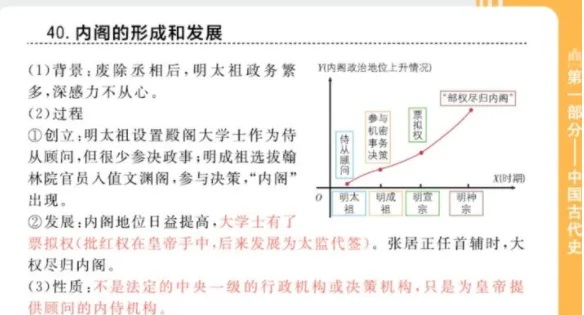
\includegraphics[width=13cm]{2024-07-30-001}
\end{figure}


如果要记忆学习上图中的明朝历史,就这么一张PPT让孩子们直接去强行背诵,那肯定是记不住的。

要是整本历史书所有知识点都要这么零散的强行背诵,这记忆量恐怕比英语还要恐怖。

\zd{别说你记不住,我也记不住。}

如果是我去讲解这东西,那我肯定要把明朝历史背后的故事讲一下,让孩子们知道明太祖为什么要创立内阁,发展的过程中有什么好玩典故,明太祖在乎什么,不在乎什么,为什么这么想。

这么上课孩子们肯定好记忆,提到明太祖就立刻能联想到这一系列的东西。

\zd{甚至不止内阁,可以把书上整个明朝所有需要背诵的知识点串起来说,找一个有趣的点作为核心链接起来,选一个好玩的视角,然后拼成长篇故事。}

\zd{你能说到让孩子们如痴如醉,听到下课铃就烦,拉着你不让你下课的地步,那你这节课的知识孩子们不费吹灰之力就能深刻记忆,举一反三,记一个点可以贯通全局。}

但如果你只是这么放PPT上讲一下,然后一切都让孩子们自己背,那孩子们必然要耗费数倍的精力才能把这东西勉强背下来,而且相当痛苦。

\zd{在孩子同样智商,同样努力的情况下,不同的授课方式会导致孩子们对这个知识点产生不同的印象,而不同的印象会带来不同的记忆难度,最终在复现知识的时候产生巨大的容量差别。}

这就是名师讲课和普通老师讲课的差别。

不能说同一个老师教课,怎么有的孩子行,你就不行,这是完全把责任甩在孩子身上了。

孩子本身固然有天赋差别,但老师确实也有差别,只不过找好老师太难,绝大多数老师都是普通人,按规定完成教学任务就完事了,能大幅降低学习难度的办法过难,\zd{知识点打碎重新组织,这种行为几乎等同于重构书本,甚至凌驾于书本,他们没动力做,也没那能力去做。}

简单的在PPT里把要背的考点列举个1234,让孩子们去死记硬背,这多简单,多容易操作,也有利于地方教育部门批量培训大量老师按这个办法展开工作。

达到我说的这种好老师地步,是绝对的凤毛麟角,比清北学生的比例还要低得多,找真正的好老师远不是一般家庭可以承受的代价,于是就只能要求孩子好好学习,不要考虑老师的差别问题。

绝大多数家庭都找不到好老师,眼下的老师即便换了,大概率也是个照本宣科的普通老师。

\zd{老师的任务就是把考点和知识点给你复述一遍,做到这一步他们就已经算完成了本职工作,能讲到学生如痴如醉的地步,那都是传说级老师,全国都没几个。}

\zd{所以当老师给你讲知识点、考点的时候,你不能直接按上课笔记硬背,你必须自己找到政治历史这类课知识点背后的共同点或者说连接点。}

也就是,所谓的历史课和政治课的低级脉络。

\zd{我没参加过文科考试,高中阶段的低级脉络我也没有感悟过,只是高屋建瓴的从高处去反推,所以我只能大概说说其中的原理,具体描述说不清楚,但这东西肯定有。}

人类大脑的缓存太低,只能记忆极少量的东西,所以会自动抛弃大脑认为不重要的部分。

比方说,你的眼睛明明看到你出门的时候是不是关门了。

但出门的1分钟后,你也许就把这件事给忘了,死活无法确认自己是否关了门,脑海中空白一片,毫无记忆。

因为你的大脑认为这个细节不重要,为了避免这东西占缓存,直接就把这段记忆给删除了,去记那些大脑认为更重要的东西。

\zd{缓存大小,直接决定了一个人的反应能力和大脑响应速度,也就是俗称的脑子转得快。}

目前绝大多数人类的缓存其实是够用的,在几十亿年的进化里,\zd{人类目前的大脑缓存,足够你逃跑用,足够捕猎用,足够你搏杀用,也足够你寻找异性繁衍后代用。}

既然完全够用,那干嘛要进化出更强的缓存?

但基因万万没想到的是,人类文明的进化速度远远超过了基因的进化速度。

基因不需要大脑去解三位数乘法,也不需要大脑去背诵滕王阁序。

\zd{整个自然界没有任何动物需要去背滕王阁序这玩意,也不需要学三位数算术,但人类需要。}

所以缓存不够用了。

不借助草稿纸,人类大脑连三位数乘法都搞不定。

不借助计算机,目前的大多数顶级数学问题人类已经彻底无能为力了,因为这些数学问题远超草稿纸可以运算的范畴。

简单说,人类大脑等于是80年代的垃圾CPU,就算运行90年代的小游戏都够呛,更别说去运行2022年的新款大型游戏了。

\zd{因此目前人类所有的所谓学习办法,记忆办法,本质上都是用那可怜的缓存,去尽可能的链接最多的知识点。}

每一个知识点的大小最多等于缓存,而链接办法的大小最多等于缓存,双方的化学反应之和等于你记忆的天赋极限长度。

有人大脑天生缓存是10KB的,有人大脑天生缓存是15KB的,双方的能力会有巨大差别,但这并不是不可弥补的。

如果你没有领悟并记忆相应脉络链接办法,那天生缓存高一点实际上根本发挥不出优势。

利用脉络,有人可以用10KB的缓存发挥出100KB乃至于1000KB的记忆力,而有的人虽有15KB的缓存,却没有任何脉络的强行死记硬背,那撑死就是15KB的记忆量,这差距简直太大了。

但如果那个拥有15KB内存的人类同时拥有坚韧的意志和对一件事情充满兴趣要研究到底的精神,深钻某个领域数年,数十年,掌握了低级,中级,乃至于高级脉络办法。

那在这个领域双方的差距就远不止50\%,可以达到100倍乃至于500倍的差距,你看对方好像是在看神,觉得对方的一切成果都不可思议。

\zd{这个领域的诸神之战,发生在那些缓存15和16KB,并且双方都投入一切精力,深耕此行业十几二十年的超级学科专家身上。}

爱因斯坦也只是在物理学上厉害,在生物学上并不比普通专家强,在菜市场还价方面甚至还不配给大妈提鞋。

没有任何专家是万能的,他们能强在一个领域就不错了,撑死就几个领域,其他领域甚至不如普通人,因为投入的时间没普通人多。

不同领域的顶级专家,也会对彼此的思考方式毫不理解,如观天书,\zd{因为他们只有在自己掌握高级脉络的领域才算专家,其他领域可能连低级脉络都没搞清楚。}

其实因为人脑缓存有限,所以所有知识密集型行业都有各自的脉络,甚至连码农应该都有。

我不清楚码农的脉络是什么,但我知道掌握低级脉络的差不多可以当码农组长/主管;掌握中级脉络的差不多可以当架构师了,制定公司软件代码工作的整体布局;掌握高级脉络的基本就是公司创始人了,引领互联网业态前进方向。

大概应该是这个样子,我不是这行人,随便估一下。

\zd{当然对于自家孩子的教育而言,低级脉络已经足够用了,这东西是可以横扫学校的大杀器,其他中高级脉络都是踏入社会后才有可能领悟并掌握的。}

不是说学生阶段完全不可能领悟,天纵奇才是可能提前领悟的,但在学生阶段领悟这些不会给你的考试分数带来丝毫助益,会让你为了领悟而耗费的时间全部白白浪费,甚至可能会出现你花费时间反而丢分的情况。

\zd{但是学生早晚会长大的,而踏入社会后就完全反过来了,低级脉络弄的再好也只能让你考试加分,对你的工资增长毫无助益,而中级脉络一旦顿悟你就可以升职加薪,能领悟高级脉络的少数人,则可以实现你期望的一切自由,成为真正的人才。}

\zd{因为任何知识密集型行业,高级脉络都极难领悟,且一定建立在至少一个中级脉络的基础上。}

\zd{希望本文蕴含的知识,能对你有所帮助。}

\end{document}

